\begin{figure}[h]
    \centering
    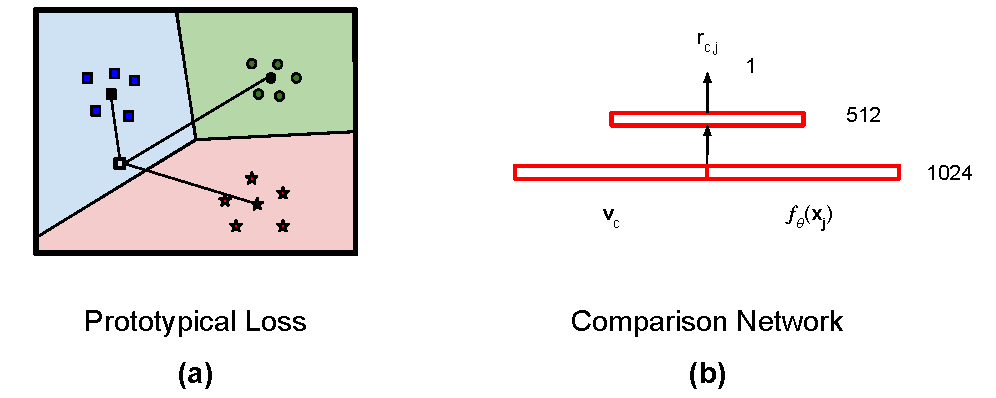
\includegraphics[width=\linewidth]{fig/meta_learning_lossfn.pdf}
    \caption{\textbf{(a)} Illustrating the training step in prototypical networks. Decision regions are indicated using background colors. For each class, prototypes are estimated as the centroid of supports (filled shapes). Given the query (unfilled shape), negative distances to each prototype are treated as logits. Adopted from \cite{koluguri2020}. (\textbf{b}) Comparison module in relation networks. The sum of support embeddings from class $c$ ($\mathbf{v}_c$) is concatenated with a query embedding ($f_\theta(\mathbf{x}_j)$) and input to the comparison network. $r_{c,j}$ is known as the relation score for query $\mathbf{x}_j$ with respect to class $c$ and treated as the logit.}
    \label{fig:metaLearningLoss}
\end{figure}

\section{Experiments and Results}
\label{sec:expts}

\subsection{Baseline Speaker Embeddings}
\label{subsec:exp_baseline}
In order to select a competitive and fair baseline to meta-learned embeddings, we first developed an implementation of x-vectors. % which have achieved the state-of-the-art performance in multiple speaker identity applications. 
Our model is similar to the Kaldi Voxceleb recipe\footnote{https://kaldi-asr.org/models/m7} with respect to training corpora and network architecture. We compare the reported performance of Kaldi embeddings with our implementation and select the best performing model as the baseline system.

As mentioned in Section \ref{subsec:data_vox}, we use the Vox2 and Vox1-dev corpora for embedding training. Similar to the Kaldi recipe, we extract 30-dimensional MFCC features using a frame width of 25ms and overlap of 15ms. We augment the training data with noise, music and babble speech using the MUSAN corpus\cite{snyder2015musan}, and reverberation using the RIR\_NOISES \footnote{\url{http://www.openslr.org/28}} corpus. The augmented data consist of 7323 speakers and 2.2M utterances. Following which, all utterances shorter than 4 seconds in duration and all speakers with fewer than 8 utterances each are removed to assist the training process. Cepstral mean normalization using a sliding window of 3 seconds was performed to remove any channel effects.

The model architecture consists of 5 time-delay layers which model temporal context information, followed by a statistical pooling layer to map into a utterance-level vector. This is followed by two feed-forward bottleneck layers with 512 units in each layer and the final layer which outputs speaker posterior probabilities. In contrast with the Kaldi implementation, we use Adam optimizer ($\beta_1$=0.9, $\beta_2$=0.99) to train the model, with an initial learning rate of 1e-3. The learning rate is increased to 2e-3 and progressively reduced to 1e-6. Dropout and batch normalization are used at all layers for regularization purpose. A minibatch of 32 samples is used at each iteration, while ensuring that utterances in each minibatch are of fixed duration to improve the training process. We accumulated gradients for every 4 minibatches before back propagation, which was observed to improve model convergence.

\begin{table}
\caption{Selecting a baseline system for speaker diarization. For each embedding and clustering method (AHC-f: AHC with fixed threshold, AHC-p: AHC with optimized threshold, bSC: binarized spectral clustering with normalized maximum eignegap), diarization error rate (DER \%) is provided for two settings: using oracle speaker count (Oracle) and estimated count (Est). }
\label{tab:spkrDiarBase}
\centering{
\begin{tabular}{ccp{6.1mm}p{6.1mm}p{6.1mm}p{6.1mm}p{6.1mm}p{6.1mm}} \hline
\multirow{2}{*}{Tool} & \multirow{2}{*}{Method} & \multicolumn{2}{c}{DIHARD} & \multicolumn{2}{c}{AMI} & \multicolumn{2}{c}{ADOSMod3} \\
 &  & Oracle & Est & Oracle & Est & Oracle & Est \\ \hline
 \rule{0pt}{2ex} 
\multirow{3}{*}{Kaldi} & AHC-f & \textbf{15.94} & 24.67 & 13.96 & 12.64 & 19.53 & 31.05 \\
 & AHC-o & - & 18.35 & - & 14.28 & - & 18.17 \\
 & bSC & 18.81 & 15.26 & 8.57 & 9.50 & 14.77 & 19.57 \\ \hdashline
 \rule{0pt}{2ex} 
\multirow{3}{*}{\begin{tabular}[c]{@{}c@{}}Ours\\ fc1\end{tabular}} & AHC-f & 17.09 & 24.47 & 15.40 & 14.49 & 18.82 & 33.14 \\
 & AHC-o & - & 18.74 & - & 14.55 & - & 20.18 \\
 & bSC & 18.81 & 14.62 & 7.95 & 14.51 & 15.85 & 21.37 \\ \hdashline
 \rule{0pt}{2ex} 
\multirow{3}{*}{\begin{tabular}[c]{@{}c@{}}Ours\\ fc2\end{tabular}} & AHC-f & 22.17 & 24.77 & 18.03 & 16.25 & 18.89 & 30.37 \\
 & AHC-o & - & 19.61 & - & 16.23 & - & 20.03 \\
 & bSC & 17.62 & \textbf{13.93} & \textbf{6.94} & \textbf{8.47} & \textbf{13.94} & \textbf{17.16} \\ \hline
\end{tabular}}
\end{table}

\subsection{Meta-learned embeddings}
\label{subsec:training_details}

%How many layers, using pre-trained TDNN layers, sanity experiment, varying the number of classes, varying number of samples per class

We select DNN architectures for the meta-learning models similar to the baseline model in order to enable a fair comparison. % to the extent possible. 
We use the same network as x-vectors except for the final layer, i.e., we retain the time-delay layers, the stats pooling layer, and two fully connected layers with 512 units in each layer. 
The protonet model uses an additional two fully connected layers with 512 units in each layer. Embeddings extracted at the final layer are used for prototype computation and loss estimation. The relation network uses one additional fully connected layer (512 units) for the encoder network. The comparison network consists of three fully connected layers with 1024 units at the input, 512 units in the hidden layer and 1 unit at the output. 
For both networks, we use batch normalization which was observed to improve convergence. We do not use dropout in the meta-learned models following their respective original implementations \cite{snell2017prototypical,sung2018learning}. The number of trainable parameters for the baseline x-vector model, protonet and relation net (encoder + comparison) are 9.8M, 6.6M and 7.1M, respectively. 
We trained both protonets and relation nets using the Adam optimizer ($\beta_1$=0.9, $\beta_2$=0.99). The initial learning rate was set to 1e-4 and exponentially decreased ($\gamma$ = 0.9) every 10 episodes, where an episode corresponds to a single back-propagation step. The models were trained for 100K episodes with the stopping point determined based on convergence of smoothed loss function. The architecture and initialization strategies for all models are presented in Figure~\ref{fig:metaLearningArch}, while the meta-learning losses are illustrated in Figure~\ref{fig:metaLearningLoss}.

\textbf{Model Initialization:}
We use a part of the pre-trained x-vector model as an initialization for the meta-learning model. 
%Specifically, we borrow the trained weights from the time-delay layers of the x-vector model. 
Specifically, we initialize the time-delay layers using the pre-trained weights from the corresponding layers from the x-vector model.
The fully connected layers are initialized uniformly at random between $[\frac{-1}{\sqrt{N}}, \frac{1}{\sqrt{N}}]$ where $N$ is the number of parameters in the layer. Empirically, we observed that the above initialization scheme provided a significant performance improvement in our experiments. 

\begin{figure*}[h]
\begin{tikzpicture}
  \node (img)  {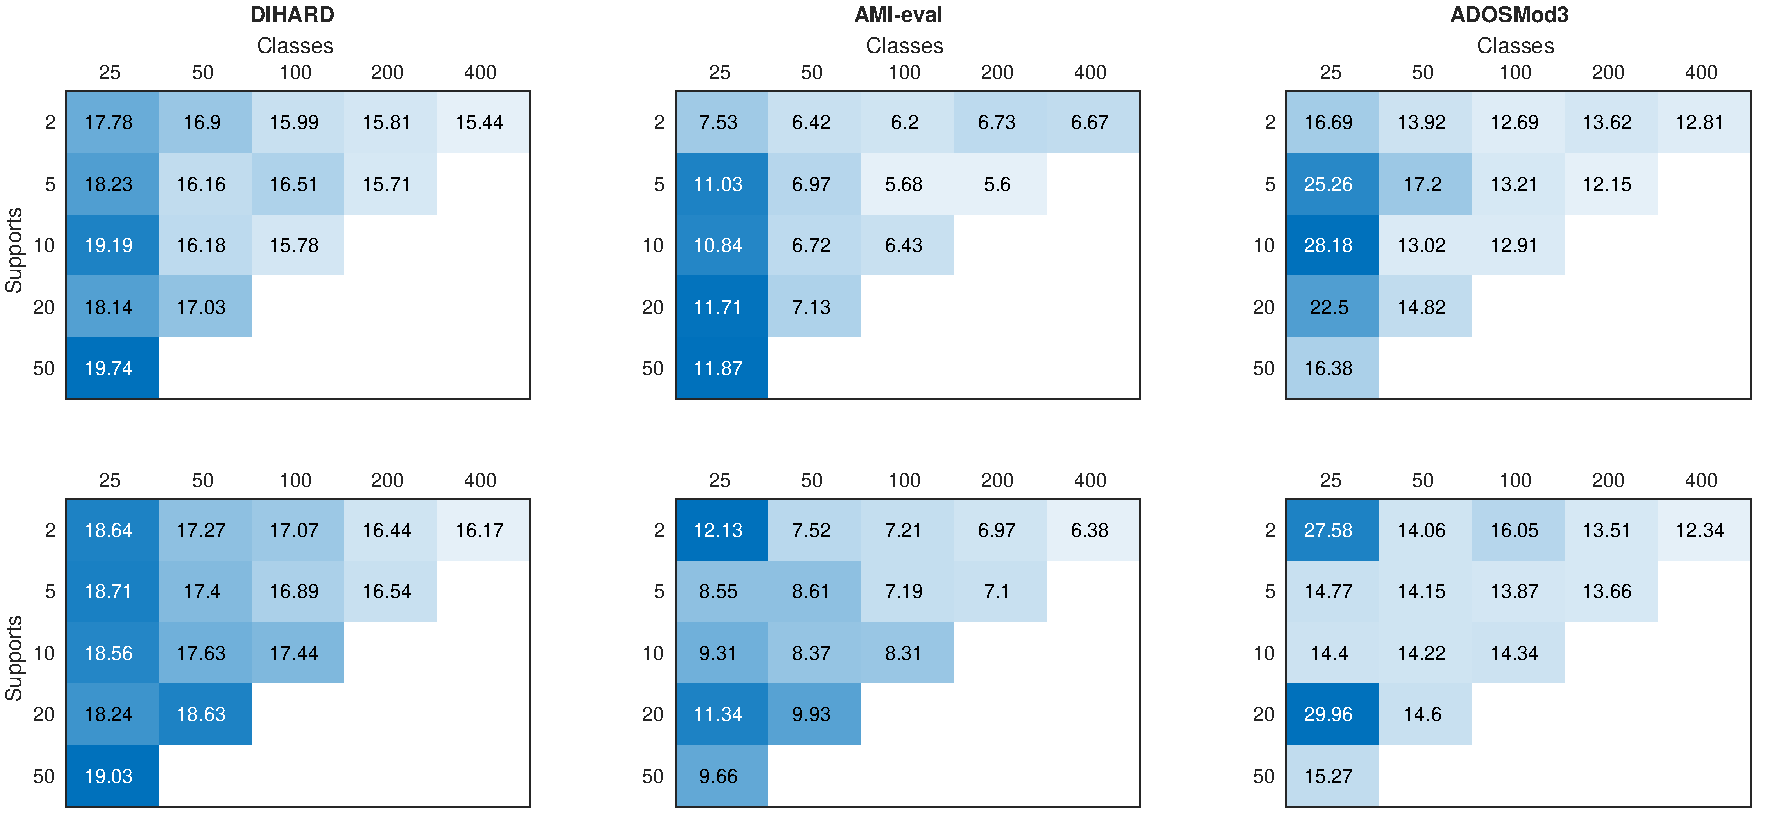
\includegraphics[width=0.9\textwidth, height=7cm]{fig/taslp_map.pdf}};
  \node[left=of img, node distance=0cm, rotate=90, anchor=center,yshift=-0.7cm] {\hspace{-1cm}  Relation Net \hskip 2.3cm Protonet};  
 \end{tikzpicture}
\caption{Speaker diarization performance (\% DER) across different corpora for different combinations of supports examples and training classes within an episode. Number of queries per class is always 1 in all experiments.}
\label{fig:wayShotExpt}
\end{figure*}

\begin{table}[h!]
\caption{Speaker diarization results comparing meta-learning models with x-vectors. x-vector+retrain represents mean DER computed with 3 trials}
\label{tab:spkrDiarCore}
\centering
\begin{tabular}{ccccccc} \\ \hline
\multirow{2}{*}{Method} & \multicolumn{2}{c}{DIHARD} & \multicolumn{2}{c}{AMI} & \multicolumn{2}{c}{ADOSMod3} \\
 & Oracle & Est & Oracle & Est & Oracle & Est \\ \hline
x-vectors & 17.62 & 13.93 & 6.94 & 8.47 & 13.94 & 17.16 \\
x-vector+retrain &  17.39 & 13.26 & 7.49 & 8.52 & 16.74 & 16.89 \\ \hdashline
\rule{0pt}{2ex}
Protonet & \textbf{15.44} & 12.96 & 6.67 & \textbf{7.31} & 12.81 & 17.22 \\ 
Relation Net & 16.17 & \textbf{12.65} & \textbf{6.38} & 8.94 & \textbf{12.34} & \textbf{16.19} \\ \hline
\end{tabular}
\end{table}

Since we borrow a part of the pre-trained x-vector model in our meta-learning models during initialization, we verify that any gains in performance obtained with meta-learning models do not arise from overtraining the x-vector model.
We conduct a sanity check experiment wherein we retrain the x-vector model similar to the meta-learning models. Specifically, we use the baseline model from Section \ref{subsec:exp_baseline} and retrain it using pre-trained weights for time-delay layers and random initialization for the fully-connected layers. The model was trained for 100K minibatches, which corresponds to the same number of episodes used for training meta-learning models.

\subsection{Speaker Diarization Results}
\label{subsec:spkrDiarResults}

We use the oracle speech activity detection for speaker diarization in order to study exclusively the speaker errors. We segment the session to be diarized into uniform segments 1.5 seconds long in duration and with an overlap of 0.75 seconds. Embedding clustering is performed using the NME-SC method as described in Section \ref{subsubsec:bSCNME}. During scoring, we do not use a collar similar to DIHARD evaluations. However, we discard speaker overlap regions since neither x-vectors nor meta-learned embeddings are trained to handle overlapping speech.

Table \ref{tab:spkrDiarBase} presents speaker diarization results for various baseline embeddings. We compare between pre-trained Kaldi embeddings, and both feed-forward bottleneck layers in our implementation. In addition to NME-SC for speaker clustering, we use AHC on PLDA scores using two methods for estimating number of speakers: (1) A fixed threshold parameter of 0, (2) Tuned threshold parameter using a development set. We tuned the parameter using two-fold cross validation for DIHARD and ADOS-Mod3, and the AMI-dev set for the AMI corpus.

\begin{figure*}[h]
    \centering
    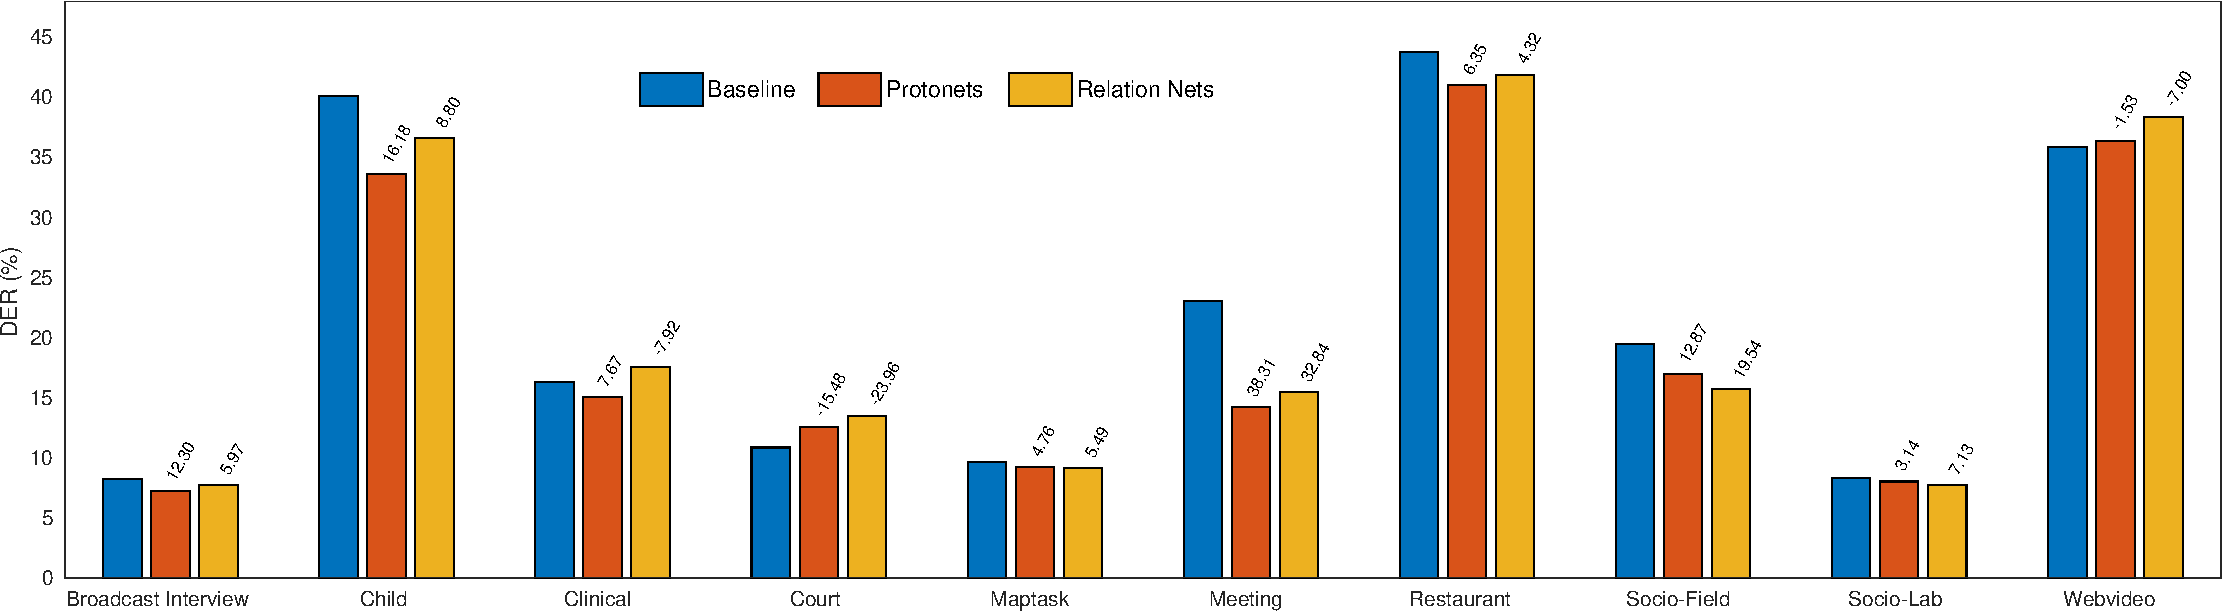
\includegraphics[width=\textwidth]{fig/taslp_bar.pdf}
    \caption{Diarization performance across domains in DIHARD. For each domain, the mean DER across sessions is provided for baseline (x-vectors), protonets and relation nets. The relative change in DER (\%) with respect to the baseline is given next to the bar (postive: DER reduction)}
    \label{tab:domain_results}
\end{figure*}

First, we notice that AHC is quite sensitive to the threshold parameter when estimating the number of speakers across all corpora and clustering methods. DER reduction using a fine-tuned threshold is particularly significant for the ADOS-Mod3 corpus with nearly 13\% absolute improvement for fc1, and 10\% for fc2 embeddings extracted using our network. 
In some cases on the DIHARD and AMI corpora the DER obtained by fine-tuning the threshold is lower than when oracle number of speakers is used, similar to observations in \cite{pal_clusterGAN2020}.
Next, fc1 embeddings outperform fc2 embeddings when clustering using AHC and PLDA scores, consistent with findings from \cite{snyder_xvec2017}. However, when cosine affinities are used with NME-SC we notice that the layer closer to the cross-entropy objective (fc2) results in a lower DER. This is the case both when oracle number of speakers are used as well as when they are estimated using the maximum eigengap value. The combination of fc2 embeddings with NME-SC method returns the lowest DERs for most conditions. Further, NME-SC removes the need for a separate development set for estimating the threshold parameter. Hence, we adopt this as the diarization baseline method in all our experiments.

In Table \ref{tab:spkrDiarCore}, we compare the baseline with the meta-learning models. \textit{x-vector+retrain} represents mean results from 3 trials of the sanity check experiment described in the Section \ref{subsec:training_details}. Both meta-learning models were trained for 100K episodes. Within each episode, 400 classes were randomly chosen without replacement from the training corpus. Following which, 3 samples were chosen without replacement from each class. Two samples were treated as supports, while the third sample was treated as query. 
%Choices for number of classes, supports and queries were constrained by GPU memory limits. 
From the results, we note that retraining the x-vector model provides minor DER improvement on the DIHARD corpus while performance worsens on the AMI corpus. The meta-learning models outperform the baselines in most cases, although improvements depend on the corpus and setting. On the DIHARD corpus consisting of challenging domains, protonets result in 12.37\% relative improvement given oracle number of speakers and 6.96 \% improvement when the number of speakers are estimated. Relation networks show a slight degradation when compared to protonets. This difference is more on a relatively clean corpus such as AMI while estimating number of speakers. 
In the following experiments, we analyze which setups contribute to improvements in performance over x-vectors.
% Compute the error in estimating number of speakers.

\subsubsection{Effect of classes within a task}

While training meta-learning models, previous works \cite{snell2017prototypical, sung2018learning, vinyals2016matching} often carefully control the number of classes (\textit{way}) within an episode and the number of supports per class (\textit{shot}) so as to match the evaluation scenario. 
Drawing analogies with speaker diarization, a typical session consists of $\mathcal{O}(1)$ speakers (\textit{way}), with $\mathcal{O}(10)$ utterances per speaker (\textit{shot}). In this experiment we vary hyper-parameters for both protonets and relation nets, and study the effect on DER. We vary the \textit{way} and \textit{shot} between 25 to 400, and 2 to 50, respectively, and train a new meta-learning model for each configuration. Results are presented in Fig~\ref{fig:wayShotExpt}. 

A common effect across different corpora and models is that the number of speakers (classes) is an important parameter for diarization performance. Increasing the number of speakers in an episode favours DER. This is similar to previous findings in few-shot image recognition \cite{snell2017prototypical}, where during training, a higher \textit{way} than expected during testing was found to provide the best results. However, the effect of supports per class on DER is not straightforward. When a large number of classes is used, increasing supports provides little to no improvements in both protonets and relation nets. Upon reducing the number of classes, the performance degrades with more supports across most models. This suggests a possibility of over-fitting due to large number of supports even though the configuration closely resembles a test session. It is more beneficial to increase the number of classes within an episode during training.

% \begin{table}[]
% \begin{tabular}{ccccccc}
% \textbf{} & \textbf{400} & \textbf{200} & \textbf{100} & \textbf{50} & \textbf{25} & \textbf{10} \\
% \textbf{2} & 15.44 & 15.81 & 15.99 & 16.90 & 17.78 & 18.94 \\
% \textbf{5} & - & 15.71 & 16.51 & 16.16 & 18.23 & 18.45 \\
% \textbf{10} & - & - & HPC & 16.02 & 19.19 & 21.56 \\
% \textbf{20} & - & - & - & HPC & 18.14 & HPC \\
% \textbf{50} & - & - & - & - & HPC & 26.09
% \end{tabular}
% \end{table}

% % \usepackage[table,xcdraw]{xcolor}
% % If you use beamer only pass "xcolor=table" option, i.e. \documentclass[xcolor=table]{beamer}
% \begin{table}[]
% \begin{tabular}{ccccccc}
% \textbf{} & \textbf{400} & \textbf{200} & \textbf{100} & \textbf{50} & \textbf{25} & \textbf{10} \\
% \textbf{2} & 6.67 & 6.73 & 6.20 & 6.42 & 7.53 & 12.23 \\
% \textbf{5} & - & 5.60 & 5.68 & 6.97 & 11.03 & 10.66 \\
% \textbf{10} & - & - & HPC & HPC & 10.84 & 21.67 \\
% \textbf{20} & - & - & - & HPC & 11.71 & HPC \\
% \textbf{50} & - & - & - & - & HPC & 25.21
% \end{tabular}
% \end{table}



\subsubsection{Performance across different domains in DIHARD}

It is often useful to understand the effect of conversation type, including speaker count, spontaneous speech and recording setups on the diarization performance. We study this using the domain labels \cite{ryant2019second} available for the DIHARD corpus. For each domain, we compute the mean DER across sessions using the baseline model as well as the meta-learning models. Oracle speaker count is used during clustering in order to exclusively study the effect of domain factors. We do not include the Audiobooks domain in this experiment since all the models return the same performance on account of sessions consisting of only one speaker.
We present the results in \mbox{Table \ref{tab:domain_results}}.

We note that there exists considerable variation between domains in terms of the DER improvement between x-vectors and meta-learning models. Broadcast news, child, maptask, meeting and socio-field domains show significant gains due to meta-learning models. Specifically, meeting and child domains benefit upto 38.31 \% and 16.18 \% relative DER improvement from protonets. Diarization in the court domain degrades in performance consistently between protonets and relation nets, with up to 20.05 \% relative degradation for relation networks. Upon a closer look at the court and meeting domains to understand this difference, we note that both domains contain similar number of speakers per session (Court: 7, Meeting: 5.3). However, the domains differ in the data collection setup: court sessions are collected by averaging audio streams from individual table-mounted microphones, while meeting sessions are collected using a single table microphone distant from all the participants \cite{ryant2019second}. Among the socio-linguistic interview domains, interviews recorded in the field under diverse locations and subject age groups (socio-field) result in a larger DER improvement over those collected under quiet conditions (socio-lab). Socio-lab contains recording from both close-talking and distant microphones, hence it is not immediately clear whether microphone placement alone is a factor in DER improvement. 
Child and restaurant domains show variation in DER reduction although they perform similar with the baseline models, suggesting that background noise types affect benefits from meta-learning.
Overall, most domains that include in-the-wild data collection show improvements with meta-learning.

\subsubsection{Performance across different child age groups}

As mentioned in Section \ref{subsec:ados}, 
automatic child speech processing has been considered a hard problem when compared to processing adult speech.
More recently, the child domain returned one of the highest DERs during the DIHARD evaluations \cite{Xie2019}, illustrating the challenges of working with child speech for diarization.
% cite this: https://pdfs.semanticscholar.org/55b8/7e974c360b8e33aa2391b2721250885aae35.pdf
Considering meta-learning models return significant improvement over x-vectors for child domain, we attempt to understand gains in DER by controlling for the age of the child. Children develop linguistic skills as they grow up, hence child age is a reasonable proxy for their linguistic development. 
We select sessions from the ADOS-Mod3 corpus where we have access to the child age metadata.
We compute the DER for each child using the respective baseline and meta-learned models described in Section~\ref{subsec:training_details}. For children where two sessions are available, we compute the mean DER per child. We study the effect of child age on DER by grouping child age into 3 groups with approximately equal number of children in each set. Children below 7.5 years of age are collected in the Low age group, children between 7.5 years and 9.5 years of age are collected in the Mid age group, and children above 9.5 years of age are collected in the High age group.

\begin{table}[h]
\caption{Analysis of child-adult diarization performance on the ADOS-Mod3 corpus. For each age group, mean DER (\%) of sessions in each group are presented along with relative improvement in parenthesis.}
\label{tab:age_expt}
\centering
\begin{tabular}{cccc} \\ \hline
Model & Low & Mid & High \\ \hline
\rule{0pt}{3ex} Baseline & 17.36 & 13.42 & 13.77 \\
\rule{0pt}{3ex} Protonet & 15.77 (9.16) & \textbf{12.39 (7.68)} & 12.33 (10.46)\\
%\rule{0pt}{2ex} \% Change (Protonet) & -9.16 & -7.68 & -10.46 \\
\rule{0pt}{3ex} Relation Net & \textbf{15.69 (9.62)} & 12.82 (4.47) & \textbf{11.37 (17.43)} \\ \hline
%\rule{0pt}{2ex} \% Change (Relation Net) & -9.62 & -4.47 & -17.43 \\ \hline
\end{tabular}
\end{table}

From the results in Table~\ref{tab:age_expt}, we notice that the Low age group returns the highest DER, while Mid and High age groups return similar performance across models. Given that children in the Low age group are more likely to exhibit speech abnormalities, this result illustrates the relative difficulty in automatic speech processing under such conditions. Improvements in DER from meta-learning models are distributed across all age groups.
A consistent improvement of 10\% relative DER among the Low age group is particularly encouraging given the challenging nature of such sessions. The high age group exhibits similar improvements in DER, with the relation networks providing upto 17.43 \% relative gains. 

\subsection{Speaker Verification Results}

We use speaker verification as another application task to illustrate the generalized speaker information captured by meta-learned embeddings. Similar to speaker diarization, we first evaluate our implementation of the baseline with the pre-trained Kaldi embeddings. We use the test partition of Voxceleb corpus, the eval set in VOiCES corpus and the eval set in SITW corpus in our experiments.
We use the core-core condition in the SITW corpus where a single speaker is present in both utterances during a trial. For all models, we score trials using PLDA after performing dimension reduction to 200 using LDA and length-normalization. The PLDA model is trained using the same data for embedding training, i.e., Vox2 corpus and the dev set of Vox1 corpus. Speakers in the SITW corpus which overlap with the Voxceleb corpus were removed from the trials before evaluation.
We use equal error rate (EER) as the metric to select the best performing baseline system. 
Since cosine scoring returned significantly high EERs relative to PLDA, we did not investigate it further.
Results are provided in Table~\ref{tab:base_sv}.

\begin{table}[h]
\caption{Selecting a baseline system for speaker verification. Results are presented as equal error rate (EER \%)}
\label{tab:base_sv}
\centering{
\begin{tabular}{cccc} \hline
Embedding & Vox1-test & VOiCES & SITW \\ \hline
Kaldi & 3.128 & 10.300 & 4.054 \\
Ours:fc1 & \textbf{2.815} & \textbf{8.591} & \textbf{3.856} \\
Ours:fc2 & 3.006 & 9.854 & 4.087 \\ \hline
\end{tabular}}
\end{table}

We notice that embeddings from both layers in our implementation outperform or closely match the Kaldi implementation. Similar to observations from Section \ref{subsec:exp_baseline} and \cite{snyder_xvec2017} fc1 embeddings fare better than fc2 embeddings when scored with PLDA. We select fc1 embeddings as the baseline speaker verification method.

% To show the generalizability of meta-learning... another application... \\ 
% Remind that we use the fc1 layer, based on observations from Section ... \\
% Mention exact LDA dimension, \\
% PLDA trained using voxceleb,\\ 
% What is EER? \\
% What is minDCF, if you choose to show it? \\
% Also, show the DET curve? - How to compute this? \\

\begin{table}[h]
\caption{Speaker verification results comparing meta-learning models with x-vectors. Results presented using EER and minDCF computed at $P_{target} = 0.01$ }
\label{tab:spkrVerCore}
\begin{tabular}{ccccccc} \\ \hline
\multirow{2}{*}{Model} & \multicolumn{2}{c}{Vox1-test} & \multicolumn{2}{c}{VOiCES} & \multicolumn{2}{c}{SITW} \\
 & EER & DCF & EER & DCF & EER & DCF  \\ \hline
\rule{0pt}{3ex} Baseline & \textbf{2.815} & 0.311 & 8.591 & 0.696 & 3.856 & 0.359 \\
\rule{0pt}{3ex} Protonets & 2.831 & \textbf{0.299} & \textbf{7.837} & \textbf{0.646} & \textbf{3.560} & \textbf{0.347} \\ 
%\rule{0pt}{2ex} \begin{tabular}[c]{@{}c@{}}\% Change \\ (Protonet)\end{tabular} & 0.57 & -4.02 & -8.78 & -7.2 & -7.68 & -3.23 \\
\rule{0pt}{3ex} Relation Net & 2.884 & 0.313 & 8.238 & 0.690 & 3.725 & 0.370 \\ \hline
%\rule{0pt}{2ex} \begin{tabular}[c]{@{}c@{}}\% Change \\ (Relation Net)\end{tabular} & 2.45 & 0.77 & -4.11 & -0.89 & -3.4 & 3.04 \\ \hline
\end{tabular}
\end{table}

When comparing meta-learning models, we use the same models developed in Section~\ref{subsec:spkrDiarResults}. In addition to EER, we present results using the minimum detection cost function (minDCF) computed at $P_{target} = 0.01$. From Table~\ref{tab:spkrDiarCore}, we note that meta-learning models outperform x-vectors in most settings except in the case of Voxceleb corpus when EER is used. Both protonets and relation nets return similar EER and minDCF for the Voxceleb corpus. Interestingly, we achieve notable improvements on the relatively more challenging corpora. Protonets provide up to 8.78\% and 7.68\% EER improvements in the VOiCES and SITW corpora, respectively, with similar improvements in minDCF. While relation nets provide better performance than x-vectors in the above corpora, they do not outperform protonets in any setting. This suggests that using a predefined distance function (namely squared Euclidean in protonets) might be beneficial overall when compared to learning a distance metric using relation networks for speaker verification application.

\begin{table*}[h]
\caption{Analysis of speaker verification based on microphone location (Near: Near-field, Far: Far-field, Obs: Fully obscured) in VOiCES corpus and level of degradation artefacts in SITW corpus}
\label{tab:spkrVerRobust}
\centering
\begin{tabular}{cccccccccccc} \\ \hline
 & \multicolumn{6}{c}{VOiCES (mic location)} &  & \multicolumn{4}{c}{SITW (degradation level)} \\ \cline{2-7} \cline{9-12}
\rule{0pt}{2ex} 
Model & \multicolumn{2}{c}{Near} & \multicolumn{2}{c}{Far} & \multicolumn{2}{c}{Obs} &  & \multicolumn{2}{c}{Low} & \multicolumn{2}{c}{High} \\
 & EER & DCF & EER & DCF & EER & DCF &  & EER & DCF & EER & DCF \\ \hline
\rule{0pt}{3ex} Baseline & 3.907 & \textbf{0.3407} & 7.311 & \textbf{0.5797} & 22.65 & 0.9375 &  & \textbf{3.401} & 0.3463 & 4.815 & 0.445 \\
\rule{0pt}{3ex} Protonets & \textbf{3.801} & 0.376 & \textbf{7.132} & 0.6337 & \textbf{20.58} & \textbf{0.9366} & & 3.537 & \textbf{0.3281} & 4.414 & \textbf{0.4268} \\
% Relative (Protonets) & -2.71 & 10.36 & -2.45 & 9.32 & -9.14 & -0.1 &  & 4 & -5.26 & -8.33 & -4.09 \\
\rule{0pt}{3ex} Relation Net & 3.872 & 0.3521 & 7.618 & 0.6282 & 21.24 & 0.9527 &  & 3.81 & 0.3467 & \textbf{4.414} & 0.4525 \\ \hline
% Relative (Relation) & -0.9 & 3.35 & 4.2 & 8.37 & -6.23 & 1.62 &  & 12.03 & 0.12 & -8.33 & 1.69
\end{tabular}
\end{table*}

\subsubsection{Robust Speaker Verification}
Since VOiCES and SITW corpora return the most improvement for speaker verification, we take a closer look at which factors benefit meta-learning. For each corpus, we make use of annotations for the microphone location and channel degradation to create new trials for speaker verification. 

In the VOiCES corpus, we collect playback recordings from rooms 3 and 4 present in the eval subset. Within these recordings, we distinguish between the utterances based on the microphone placement with respect to the loudspeaker (audio source). Specifically, we create three categories: (1) utterances collected using mic1 and mic18 are treated as near-field, being closest to the source, (2) utterances collected from mic19 are treated as far-field, and (3) utterances collected from mic12 are treated as obscured, since they are fully obscured by the wall. 
While creating the trials for each category, we ensure that the ratio of target to nontarget pairs remain approximately equal to the overall eval set trial. An example room configuration is presented in Figure~\ref{fig:voicesRoom}.

\begin{figure}[h]
    \centering
    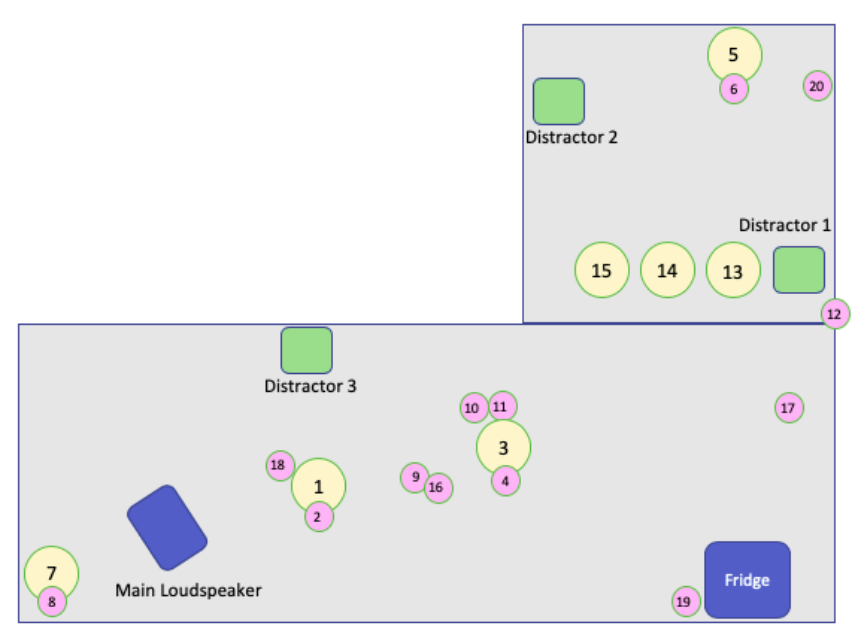
\includegraphics[scale=0.27]{fig/voices_room.png}
    \caption[An example room configuration from the VOiCES corpus]{An example room configuration from the VOiCES corpus\protect\footnotemark. Microphones are represented using circles. }
    \label{fig:voicesRoom}
\end{figure}
% Below footnote is linked to caption in fig:voicesRoom - based on https://tex.stackexchange.com/questions/10181/using-footnote-in-a-figures-caption
\footnotetext{Figure adapted from https://voices18.github.io/rooms/}

From the SITW corpus, we use the metadata annotations for level of degradation. The corpus includes multiple degradation artifacts: reverberation, noise, compression, etc, among others. The level of degradation for the most prominent artefact was annotated manually on a scale of 0 (least) to 4 (maximum). We use the trials available as part of the eval set which are annotated with the degradation level. We group the trials into two levels: low (deg0 and deg1) and high (deg3 and deg4). Note that the utterances contain multiple types of degradation in each level. 
Details of target and imposter pairs for SITW corpus (degradation level) and VOiCES corpus (microphone placement) are present in Table~\ref{tab:spkrVerDataStats}. Speaker verification results using EER and minDCF are presented in Table~\ref{tab:spkrVerRobust}.

We notice that no single model performs the best across multiple conditions. When controlled for microphone placement in VOiCES, protonets return the best EER at all locations. The margin of improvement remains approximately the same when only the distance from source is considered: 2.71\% for near-field and 2.45\% for far-field. The margin improves to 9.14\% when the microphone is fully obscured by a wall and placed close to distractor noises. Interestingly, these improvements are not reflected in the minDCF scores in the absence of noise, where x-vectors outperform both meta-learning models. %\textbf{(link this sentence to the DET curve)}. 
We believe that improvements in EER and minDCF in VOiCES corpus primarily arise from utterances collected in obstructed locations and in close vicinity of distractor noises. The experiments in SITW corpus focus on the strength of such noise conditions. Under low degradation levels, we see that x-vectors return the least EER, although their performance is not consistent with minDCF. Meta-learning models continue to work better in higher degradation levels, providing 8.3\% reduction in 4.1\% reduction in EER and minDC, respectively. %\textbf{Also, check for type of degradation level, if available?}
%\textbf{Add the Kaldi DET curves for these expts}

% \subsubsection{Dependence on utterance duration, possibly both enroll and test}
% Here we can possibly have a 2-D matrix with EER (or improvement from x-vectors?) across enroll and test utterance durations from one of the corpora where we got significant improvement.

% \subsection{Score Fusion}
% If this is ever a possibility, check out https://sites.google.com/site/bosaristoolkit/


